\documentclass[12pt,twoside]{article}
\usepackage[dvipsnames]{xcolor}
\usepackage{tikz,graphicx,amsmath,amsfonts,amscd,amssymb,bm,cite,epsfig,epsf,url}
\usepackage[hang,flushmargin]{footmisc}
\usepackage[colorlinks=true,urlcolor=blue,citecolor=blue]{hyperref}
\usepackage{amsthm,multirow,wasysym,appendix}
\usepackage{array,subcaption} 
% \usepackage[small,bf]{caption}
\usepackage{bbm}
\usepackage{pgfplots}
\usetikzlibrary{spy}
\usepgfplotslibrary{external}
\usepgfplotslibrary{fillbetween}
\usetikzlibrary{arrows,automata}
\usepackage{thmtools}
\usepackage{blkarray} 
\usepackage{textcomp}
\usepackage[left=0.8in,right=1.0in,top=1.0in,bottom=1.0in]{geometry}

\usepackage{times}
\usepackage{amsfonts}
\usepackage{amsmath}
%\usepackage[psamsfonts]{amssymb}
\usepackage{latexsym}
\usepackage{color}
\usepackage{graphics}
\usepackage{enumerate}
\usepackage{amstext}
\usepackage{blkarray}
\usepackage{url}
\usepackage{epsfig}
\usepackage{bm}
\usepackage{hyperref}
\hypersetup{
    colorlinks=true,
    linkcolor=blue,
    filecolor=magenta,      
    urlcolor=blue,
}
\usepackage{mathtools}
\usepackage{minted}
%% Probability operators and functions
%
% \def \P{\mathrm{P}}
\def \P{\mathrm{P}}
\def \E{\mathrm{E}}
\def \Var{\mathrm{Var}}
\let\var\Var
\def \Cov {\mathrm{Cov}} \let\cov\Cov
\def \MSE {\mathrm{MSE}} \let\mse\MSE
\def \sgn {\mathrm{sgn}}
\def \R {\mathbb{R}}
\def \C {\mathbb{C}}
\def \N {\mathbb{N}}
\def \Z {\mathbb{Z}}
\def \cV {\mathcal{V}}
\def \cS {\mathcal{S}}
\DeclareMathOperator*{\argmin}{arg\,min}
\DeclareMathOperator*{\argmax}{arg\,max}
\newcommand{\red}[1]{\textcolor{red}{#1}}
\newcommand{\blue}[1]{\textcolor{blue}{#1}}
\newcommand{\green}[1]{\textcolor{ForestGreen}{ #1}}
\newcommand{\fuchsia}[1]{\textcolor{RoyalPurple}{ #1}}

%
%% Probability distributions
%
%\def \Bern    {\mathrm{Bern}}
%\def \Binom   {\mathrm{Binom}}
%\def \Exp     {\mathrm{Exp}}
%\def \Geom    {\mathrm{Geom}}
%\def \Norm    {\mathcal{N}}
%\def \Poisson {\mathrm{Poisson}}
%\def \Unif    {\mathrm {U}}
%
\newcommand{\bdb}[1]{\textcolor{red}{#1}}

\newcommand{\ml}[1]{\mathcal{ #1 } }
\newcommand{\wh}[1]{\widehat{ #1 } }
\newcommand{\wt}[1]{\widetilde{ #1 } }
\newcommand{\conj}[1]{\overline{ #1 } }
\newcommand{\rnd}[1]{\tilde{ #1 } }
\newcommand{\rv}[1]{ \rnd{ #1}  }
\newcommand{\rx}{\rnd{ x}  }
\newcommand{\ry}{\rnd{ y}  }
\newcommand{\ra}{\rnd{ a}  }
\newcommand{\rb}{\rnd{ b}  }
\newcommand{\rpc}{\widetilde{ pc}  }

\def \cnd {\, | \,}
\def \Id { I }
\def \J {\mathbf{1}\mathbf{1}^T}

\newcommand{\op}[1]{\operatorname{#1}}
\newcommand{\setdef}[2]{ := \keys{ #1 \; | \; #2 } }
\newcommand{\set}[2]{ \keys{ #1 \; | \; #2 } }
\newcommand{\sign}[1]{\op{sign}\left( #1 \right) }
\newcommand{\trace}[1]{\op{tr}\left( #1 \right) }
\newcommand{\tr}[1]{\op{tr}\left( #1 \right) }
\newcommand{\inv}[1]{\left( #1 \right)^{-1} }
\newcommand{\abs}[1]{\left| #1 \right|}
\newcommand{\sabs}[1]{| #1 |}
\newcommand{\keys}[1]{\left\{ #1 \right\}}
\newcommand{\sqbr}[1]{\left[ #1 \right]}
\newcommand{\sbrac}[1]{ ( #1 ) }
\newcommand{\brac}[1]{\left( #1 \right) }
\newcommand{\bbrac}[1]{\big( #1 \big) }
\newcommand{\Bbrac}[1]{\Big( #1 \Big)}
\newcommand{\BBbrac}[1]{\BIG( #1 \Big)}
\newcommand{\MAT}[1]{\begin{bmatrix} #1 \end{bmatrix}}
\newcommand{\sMAT}[1]{\left(\begin{smallmatrix} #1 \end{smallmatrix}\right)}
\newcommand{\sMATn}[1]{\begin{smallmatrix} #1 \end{smallmatrix}}
\newcommand{\PROD}[2]{\left \langle #1, #2\right \rangle}
\newcommand{\PRODs}[2]{\langle #1, #2 \rangle}
\newcommand{\der}[2]{\frac{\text{d}#2}{\text{d}#1}}
\newcommand{\pder}[2]{\frac{\partial#2}{\partial#1}}
\newcommand{\derTwo}[2]{\frac{\text{d}^2#2}{\text{d}#1^2}}
\newcommand{\ceil}[1]{\lceil #1 \rceil}
\newcommand{\Imag}[1]{\op{Im}\brac{ #1 }}
\newcommand{\Real}[1]{\op{Re}\brac{ #1 }}
\newcommand{\norm}[1]{\left|\left| #1 \right|\right| }
\newcommand{\norms}[1]{ \| #1 \|  }
\newcommand{\normProd}[1]{\left|\left| #1 \right|\right| _{\PROD{\cdot}{\cdot}} }
\newcommand{\normTwo}[1]{\left|\left| #1 \right|\right| _{2} }
\newcommand{\normTwos}[1]{ \| #1  \| _{2} }
\newcommand{\normZero}[1]{\left|\left| #1 \right|\right| _{0} }
\newcommand{\normTV}[1]{\left|\left| #1 \right|\right|  _{ \op{TV}  } }% _{\op{c} \ell_1} }
\newcommand{\normOne}[1]{\left|\left| #1 \right|\right| _{1} }
\newcommand{\normOnes}[1]{\| #1 \| _{1} }
\newcommand{\normOneTwo}[1]{\left|\left| #1 \right|\right| _{1,2} }
\newcommand{\normF}[1]{\left|\left| #1 \right|\right| _{\op{F}} }
\newcommand{\normLTwo}[1]{\left|\left| #1 \right|\right| _{\ml{L}_2} }
\newcommand{\normNuc}[1]{\left|\left| #1 \right|\right| _{\ast} }
\newcommand{\normOp}[1]{\left|\left| #1 \right|\right|  }
\newcommand{\normInf}[1]{\left|\left| #1 \right|\right| _{\infty}  }
\newcommand{\proj}[1]{\mathcal{P}_{#1} \, }
\newcommand{\diff}[1]{ \, \text{d}#1 }
\newcommand{\vc}[1]{\boldsymbol{\vec{#1}}}
\newcommand{\rc}[1]{\boldsymbol{#1}}
\newcommand{\vx}{\vec{x}}
\newcommand{\vy}{\vec{y}}
\newcommand{\vz}{\vec{z}}
\newcommand{\vu}{\vec{u}}
\newcommand{\vv}{\vec{v}}
\newcommand{\vb}{\vec{\beta}}
\newcommand{\va}{\vec{\alpha}}
\newcommand{\vaa}{\vec{a}}
\newcommand{\vbb}{\vec{b}}
\newcommand{\vg}{\vec{g}}
\newcommand{\vw}{\vec{w}}
\newcommand{\vh}{\vec{h}}
\newcommand{\vnu}{\vec{\nu}}
\newcommand{\rvnu}{\vc{\nu}}

\newtheorem{theorem}{Theorem}[section]
% \declaretheorem[style=plain,qed=$\square$]{theorem}
\newtheorem{corollary}[theorem]{Corollary}
\newtheorem{definition}[theorem]{Definition}
\newtheorem{lemma}[theorem]{Lemma}
\newtheorem{remark}[theorem]{Remark}
\newtheorem{algorithm}[theorem]{Algorithm}

% \theoremstyle{definition}
%\newtheorem{example}[proof]{Example}
%\declaretheorem[style=definition,qed=$\triangle$,sibling=definition]{example}
%\declaretheorem[style=definition,qed=$\bigcirc$,sibling=definition]{application}

%
%% Typographic tweaks and miscellaneous
%\newcommand{\sfrac}[2]{\mbox{\small$\displaystyle\frac{#1}{#2}$}}
%\newcommand{\suchthat}{\kern0.1em{:}\kern0.3em}
%\newcommand{\qqquad}{\kern3em}
%\newcommand{\cond}{\,|\,}
%\def\Matlab{\textsc{Matlab}}
%\newcommand{\displayskip}[1]{\abovedisplayskip #1\belowdisplayskip #1}
%\newcommand{\term}[1]{\emph{#1}}
%\renewcommand{\implies}{\;\Rightarrow\;}

% My macros

\def\Kset{\mathbb{K}}
\def\Nset{\mathbb{N}}
\def\Qset{\mathbb{Q}}
\def\Rset{\mathbb{R}}
\def\Sset{\mathbb{S}}
\def\Zset{\mathbb{Z}}
\def\squareforqed{\hbox{\rlap{$\sqcap$}$\sqcup$}}
\def\qed{\ifmmode\squareforqed\else{\unskip\nobreak\hfil
\penalty50\hskip1em\null\nobreak\hfil\squareforqed
\parfillskip=0pt\finalhyphendemerits=0\endgraf}\fi}

%\DeclareMathOperator*{\E}{\rm E}
%\DeclareMathOperator*{\argmax}{\rm argmax}
%\DeclareMathOperator*{\argmin}{\rm argmin}
%\DeclareMathOperator{\sgn}{sign}
\DeclareMathOperator{\supp}{supp}
\DeclareMathOperator{\last}{last}
%\DeclareMathOperator{\sign}{\sgn}
\DeclareMathOperator{\diag}{diag}
\providecommand{\abs}[1]{\lvert#1\rvert}
\providecommand{\norm}[1]{\lVert#1\rVert}
\def\vcdim{\textnormal{VCdim}}
\DeclareMathOperator*{\B}{\textbf{B}}

%\DeclarePairedDelimiter\ceil{\lceil}{\rceil}
%\DeclarePairedDelimiter\floor{\lfloor}{\rfloor}

\newcommand{\cX}{{\mathcal X}}
\newcommand{\cY}{{\mathcal Y}}
\newcommand{\cA}{{\mathcal A}}
\newcommand{\ignore}[1]{}
\newcommand{\bi}{\begin{itemize}}
\newcommand{\ei}{\end{itemize}}
\newcommand{\be}{\begin{enumerate}}
\newcommand{\ee}{\end{enumerate}}
\newcommand{\bd}{\begin{description}}
\newcommand{\ed}{\end{description}}
\newcommand{\h}{\widehat}
\newcommand{\e}{\epsilon}
\newcommand{\mat}[1]{{\mathbf #1}}
%\newcommand{\R}{\mat{R}}
\newcommand{\0}{\mat{0}}
\newcommand{\M}{\mat{M}}

\newcommand{\D}{\mat{D}}
\renewcommand{\r}{\mat{r}}
\newcommand{\x}{\mat{x}}
\renewcommand{\u}{\mat{u}}
\renewcommand{\v}{\mat{v}}
\newcommand{\w}{\mat{w}}
\renewcommand{\H}{\text{0}}
\newcommand{\T}{\text{1}}
%\newcommand{\set}[1]{\{#1\}}
\newcommand{\xxi}{{\boldsymbol \xi}}
\newcommand{\ssigma}{{\boldsymbol \sigma}}
\newcommand{\Alpha}{{\boldsymbol \alpha}}
\newcommand{\tts}{\tt \small}
\newcommand{\hint}{\emph{hint}}
\newcommand{\matr}[1]{\bm{#1}}     % ISO complying version
\newcommand{\vect}[1]{\bm{#1}} % vectors

%\newcommand{\Var}{\mathrm{Var}}
%\newcommand{\Cov}{\mathrm{Cov}}

% New commands
\newcommand{\SP}{\mathbf{S}_{+}^n}
\newcommand{\Proj}{\mathcal{P}_{\mathcal{S}}}
\DeclarePairedDelimiterX{\inp}[2]{\langle}{\rangle}{#1, #2}
\newtheorem{proof}{Proof}


\begin{document}

\noindent DS-GA.1013 Mathematical Tools for Data Science \\
Homework 2 \\
Yves Greatti - yg390\\

\begin{enumerate}
\item (Correlation coefficient) The entries of a two-dimensional random vector have a correlation coefficient equal to one. What is the variance of the second principal component? Provide both a proof and an intuitive justification. 

Let X and Y the two components of a random vector. If $\rho_{X,Y} = \frac {\Cov(X,Y)}{\sigma_X \sigma_Y} = 1$ then $\Cov(X,Y) = \sigma_X \sigma_Y$
The covariance matrix  is then  $ \Sigma = \begin{bmatrix} \sigma_X^2 & \Cov(X,Y) \\  \Cov(X,Y) & \sigma_Y^2  \end{bmatrix}  = \begin{bmatrix}  \sigma_X^2 &  \sigma_X \sigma_Y \\ \sigma_X \sigma_Y & \sigma_Y^2 \end{bmatrix}$.
$\det(\Sigma -\lambda I) = \lambda (\lambda - (\sigma_X^2 +  \sigma_Y^2)), \lambda \in   \mathbf{R} \Rightarrow $ the eigenvalues are $0$ and $\sigma_X^2 +  \sigma_Y^2$.
The sample variance of the second principal component is the smaller eigenvalue $0$. We can expect such result since there $X$ and $Y$ are positively correlated with a coefficient of one thus the variance of the data is completely expressed by the variance of the first principal component, there is no information on the second principal component.


\newpage
\item (Not centering) To analyze what happens if we apply PCA without centering, let $\rx$ be a $d$-dimensional vector with mean $\mu \in \R^{d}$ and covariance matrix $\Sigma_{\rx}$ equal to the identity matrix. If we compute the eigendecomposition of the matrix $\E(\rx \rx^T)$ what is the value of the largest eigenvalue? What is the direction of the corresponding eigenvector? 
  
 \newpage
  
 \item (Financial data) In this exercise you will use the code in the findata folder.
  For the data loading code to work properly, make sure you
  have the pandas Python package installed on your system.

  Throughout, we will be using the data obtained by calling
 \emph{load\_data} in \emph{findata\_tools.py}.  This will
  give you the names, and closing prices for a set of 18 stocks over a
  period of 433 days ordered chronologically.
  For a fixed stock (such as msft), let
  $P_1,\ldots,P_{433}$ denote its sequence of closing prices ordered in
  time.  For that stock, define the daily returns series $R_i:=P_{i+1}-P_i$ for
  $i=1,\ldots,432$.  Throughout we think of the daily stock returns as features,
  and each day (but the last) as a separate datapoint in $\R^{18}$.
  That is, we have $432$ datapoints each having $18$ features.
  \begin{enumerate}
  \item Looking at the first two principal directions of the
    centered data, give the two stocks with the largest
    coefficients (in absolute value) in each direction.  
    Give a hypothesis why these two stocks have the largest
    coefficients, and confirm your hypothesis using the data.  The file 
   \emph{findata\_tools.py} has\emph{pretty\_print}
    functions that can help you output your results.
    You are not required to include the principal directions in
    your submission.\\ \\
    The two stocks corresponding to the two principal directions of the centered data with the largest coefficients (in absolute value) in each direction
    are: "amzn" and  "goog". It can be explained by computing the absolute return for each stock over the period of 433 days:

	\begin{figure}[H]
		\centering
		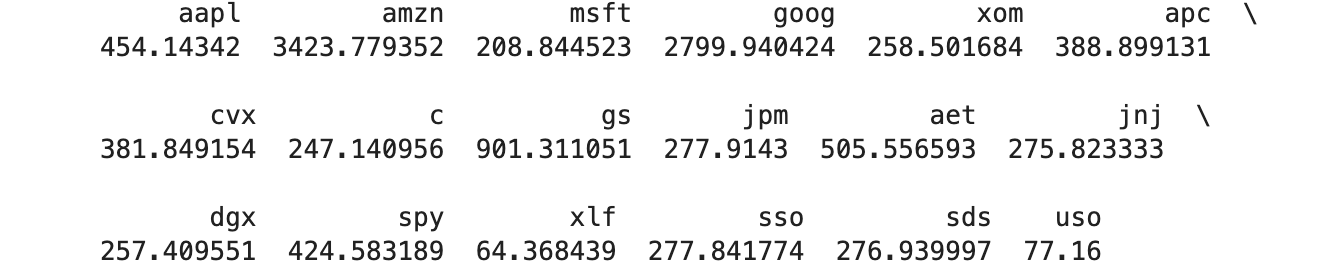
\includegraphics[width=200pt]{figures/pb_3_a.png}
		\caption{Stocks returns over a period of 433 days (output of pretty\_print).}
		\label{fig1}
	\end{figure}
    
    In term of return goog and amzn stocks returned about 4 and  3 times more than the next stock after amzn and goog stocks with the highest return: gs, 53 and 43 times more than
    the last stock in term of return among the 18 stocks: xlf.
    \begin{center}
    		\begin{tabular}{ | c | c | c | c | }
    		\hline
			\text{amzn/gs} & \text{amzn/xlf} & \text{goog/gs}  & \text{goog/xlf} \\
		\hline
			3.8 & 53.2 & 3.1 & 43.5  \\ 
		\hline
    	\end{tabular}
    \end{center}
   So most of the variance in the data will be explained by these two stocks: goog and amzn.

  \item Standardize the centered data so that each stock (feature) has
    variance 1 and compute the first 2 principal directions.  This is
    equivalent to computing the principal directions of the
    correlation matrix (the previous part used the covariance
    matrix).  Using the information in the comments of
   \emph{generate\_findata.py} as a guide to the stocks, 
    give an English interpretation of the first 2 principal directions
    computed here. 
    You are not required to include the principal directions in
    your submission.
     
    We can think of each of the entries of the principal directions as a weighting on the corresponding stock.  
    	\bi
    		\item SPY - A security that roughly tracks the S\&P 500, a weighted average of the stock prices of 500 top US companies.
		We have only 18 stocks and excluding the ETF (Exchange traded products), we are left with 13 stocks. 
		Computing the  weighted average using the entries in the first principal direction, we obtain a weighted average price
		in the range of the SPY price reported for the same day. It is less true using the entries of the second principal direction.
		
		\begin{figure}[H]
			\centering
			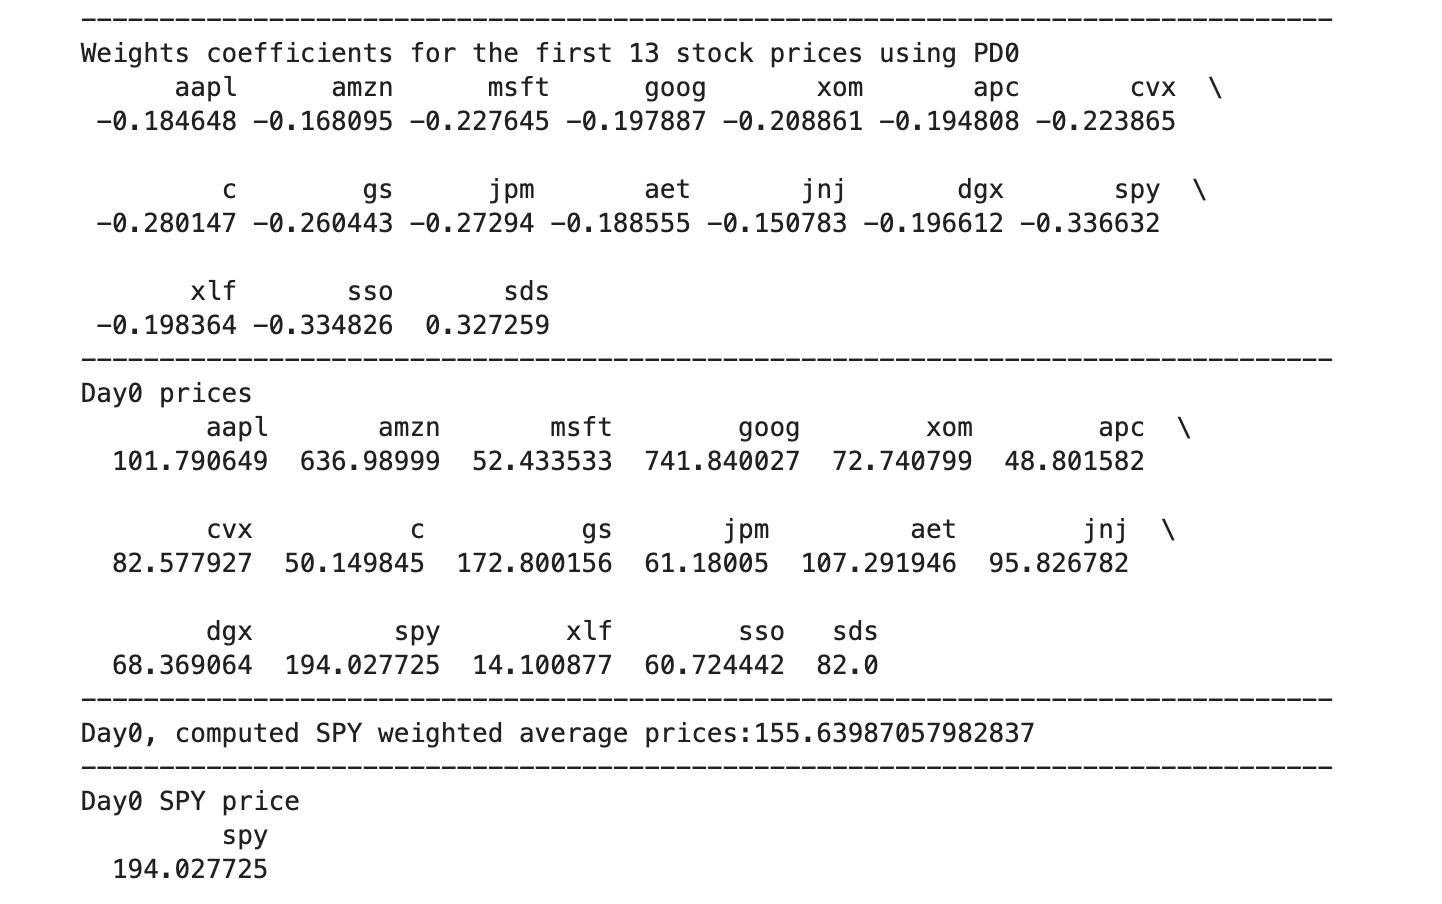
\includegraphics[width=200pt]{figures/pb_3_b_1.png}
			\caption{Weighted average of the 13 stock prices and SPY price using PD0.}
			\label{fig2}
		\end{figure}
			
		\begin{figure}[H]
			\centering
			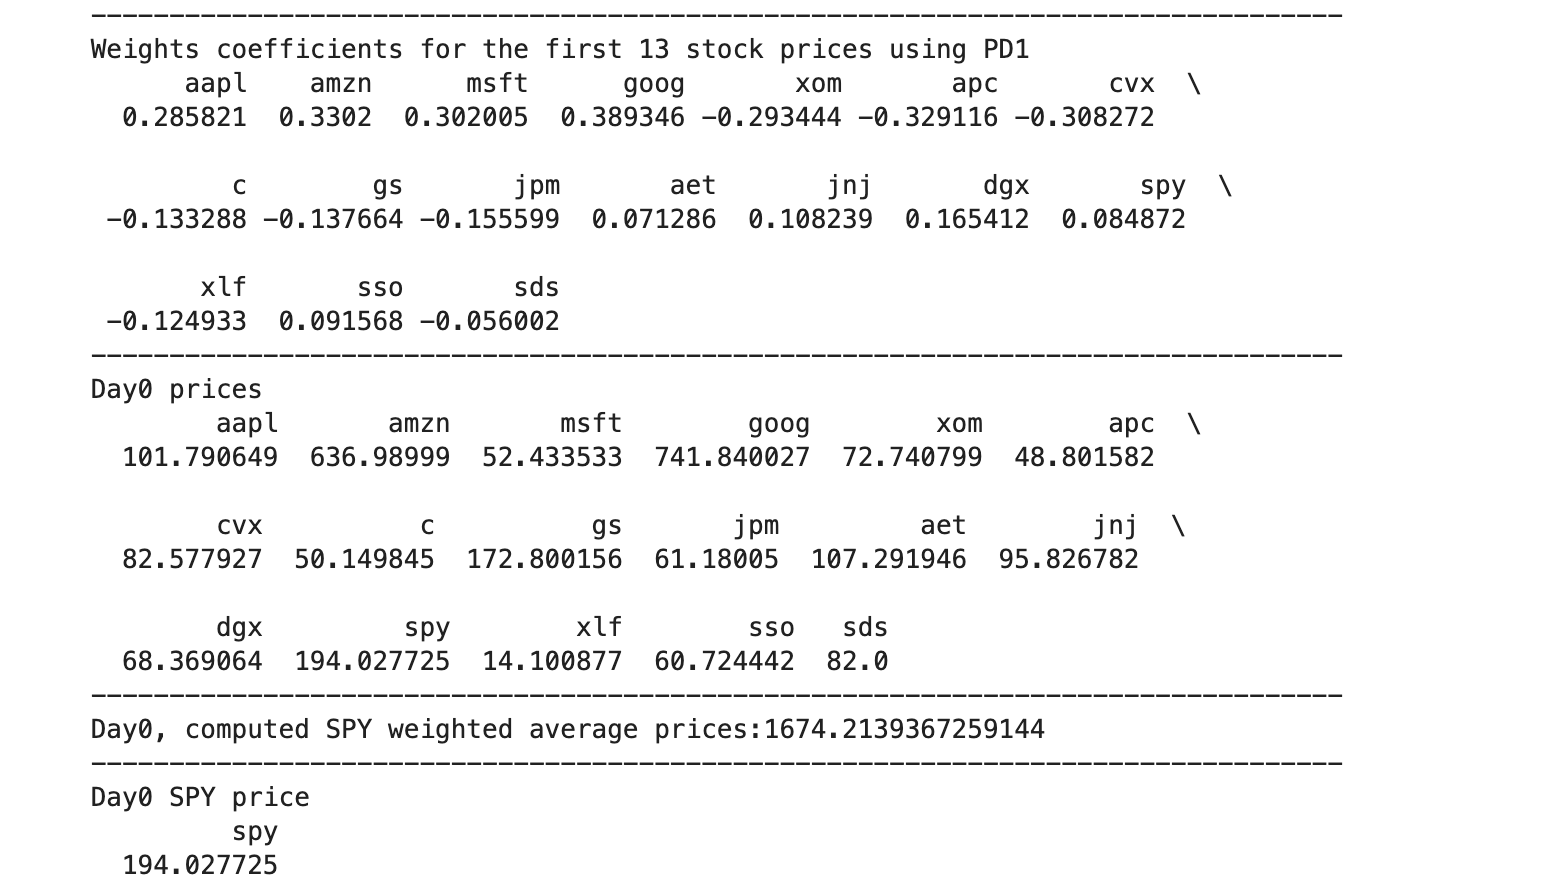
\includegraphics[width=200pt]{figures/pb_3_b_2.png}
			\caption{Weighted average of the 13 stock prices and SPY price using PD1.}
			\label{fig3}
		\end{figure}
			
		\item  XLF -  A security that tracks a weighted average of top US financial companies.
		We find the same weighting scheme but to a less extent as we have only 3 financial stocks among the 18 stocks.
		
		\begin{figure}[H]
			\centering
			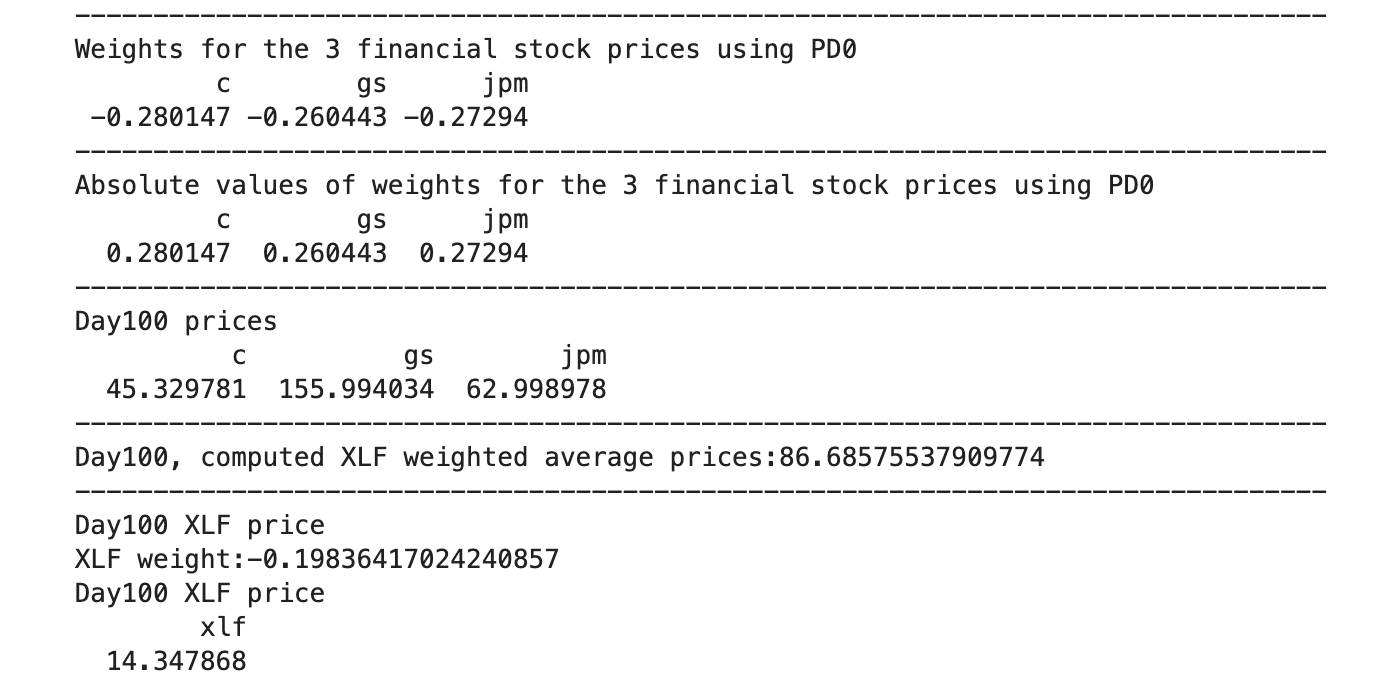
\includegraphics[width=200pt]{figures/pb_3_b_3.png}
			\caption{Weighted average of the 3 financial stock prices and XLF price using PD0.}
			\label{fig3}
		\end{figure}
	
		\item SSO - ProShares levered ETF that roughly corresponds to twice the daily performance of the S\&P 500.
		We have similar entries for SSO and SPY which indicate a strong correlation between these two stocks
		\begin{center}
    			\begin{tabular}{ | c | c | c | }
    			\hline
								& \text{SSO} 	& \text{SPY} \\
			\hline
				\text{First PD}		& -0.3348		& -0.3366  \\ 
    			\hline
				\text{Second PD}	& 0.09156		& 0.0848  \\ 
			\hline
    			\end{tabular}
   		 \end{center}
		 
		\item SDS - ProShares inverse levered ETF that roughly corresponds to twice the negative daily performance of the S\&P 500. 
		The entries for SDS and SPY are roughly opposite confirming the opposite trend of SDS compared to SPY.
		\begin{center}
    			\begin{tabular}{ | c | c | c | }
    			\hline
								& \text{SDS} 	& \text{SPY} \\
			\hline
				\text{First PD}		& 0.3272		& -0.3366  \\ 
    			\hline
				\text{Second PD}	& -0.0560		& 0.0848  \\ 
			\hline
    			\end{tabular}
   		 \end{center}
		 
		\item USO - Exchange traded product that tracks the price of oil in the US
		Taking the mean of the entries related to oil company (xom, apc, cvx) from the principal directions  and comparing to the entry for USO, they are close,
		confirming the correlation between uso and (xom, apc, cvx):
		\begin{center}
    			\begin{tabular}{ | c | c | c | }
    			\hline
								& \text{USO} 	& \text{Mean(XOM, APC, CVX)} \\
			\hline
				\text{First PD}		& -0.1592		& -0.2091 \\ 
    			\hline
				\text{Second PD}	& -0.3709		& -0.3102  \\ 
			\hline
    			\end{tabular}
   		 \end{center}
		

   	\ei
     
    
  \item Assume the stock returns each day are drawn independently from a
    multivariate distribution $\rx$ where
    $\rx[i]$ corresponds to the $i$th stock.  Assume further that
    you hold a portfolio with $200$ shares of each of appl, amzn, msft, and
    goog, and $100$ shares of each of the remaining 14 stocks in the
    dataset.  Using the sample covariance matrix as an estimator for
    the true covariance of $\rx$, approximate the standard deviation of
    your 1 day portfolio returns $\ry$ (this is a measure of the risk of your
    portfolio).  Here $\ry$ is given by
    $$\ry := \sum_{i=1}^{18} \alpha[i] \rx[i],$$
    where $\alpha[i]$ is the number of shares you hold of stock $i$.  
    
    Using the sample covariance matrix and taking the root square of [$ \text{shares}^T \times \text{covariance} \times \text{shares}$], we find that for such portfolio the standard deviation of 1 day is: $4309.94952$.
    
  \item Assume further that $\rx$ from the previous part has a
    multivariate Gaussian distribution.  Compute the probability
    of losing $1000$ or more dollars in a single day.  That is,
    compute
    $$\Pr(\ry \leq -1000).$$
    For each day of the $432$ days, we compute the daily return $\ry := \sum_{i=1}^{18} \alpha[i] \rx[i]$ and count the number of times over the $432$ days: $\Pr(\ry \leq -1000)$, then divide the result by the number of days (432),
    we obtain: $0.3425$.
    
  \end{enumerate}
  Note: The assumptions made in the previous parts are often
  invalid and can lead to inaccurate risk calculations in real
  financial situations. 
  
  \item Faces
  	\bi
		\item 
		The data set consists in $400$ rows of a ravelled face image of original size 64 x 64 pixels . Each row represent a datapoint in $\R^{4096}$.
		A label is associated to each face image which correspond to the Subject IDs.
		%The \emph{nearest_neighbors} function we compute the distance between a test image and a set of reference image (train\_matrix).
		
	\ei	
  
\end{enumerate}
\end{document}
